\chapter{Theoretical Background}\label{chap:theory}
\section{Sheet Metal Formability}
Sheet metal formability describes the ability of a sheet material to undergo plastic deformation during a forming operation without the occurrence of defects such as localized necking, fracture, wrinkling, or excessive thinning. It is a key consideration in the design of sheet metal components and forming processes, particularly in industries such as automotive, aerospace, and consumer goods manufacturing, where lightweight structures and complex geometries are increasingly required.

The formability of a sheet metal depends on a combination of material, geometrical, and process-related factors. Material properties such as yield strength, strain hardening behaviour, strain-rate sensitivity, anisotropy, and ductility directly influence the material's ability to accommodate plastic deformation. In addition, sheet thickness, tooling geometry, lubrication conditions, and the applied loading path can significantly affect the deformation behaviour and the onset of failure.

During a forming operation, deformation is rarely uniaxial and is generally characterized by a combination of major and minor in-plane strains. Different strain paths can lead to significantly different forming limits, even for the same material. Consequently, the characterization of sheet metal formability requires an approach capable of accounting for a wide range of deformation states.

Several methods have been developed to assess formability, including tensile tests, bulge tests, and standardized forming experiments. Among these, the Forming Limit Diagram (FLD) has become the most widely used engineering tool for describing the onset of localized necking under different strain paths. The FLD provides a graphical representation of the strain combinations that a material can withstand before instability occurs and forms the basis for the evaluation of sheet metal formability in both experimental and numerical investigations.

\section{Forming Limit Diagram}

The Forming Limit Diagram (FLD) is the most widely used tool for characterizing the formability of sheet metals. It plots the major principal strain, $\varepsilon_1$, against the minor principal strain, $\varepsilon_2$, at the onset of localized necking. The resulting Forming Limit Curve (FLC) defines the boundary between stable and unstable deformation. Strain states below the FLC correspond to safe deformation, whereas strain states above the curve indicate the onset of localized necking and, ultimately, fracture.

Figure~\ref{fig:FLD_example} illustrates a typical FLD and the corresponding deformation regions. The shape and position of the FLC depend on several factors, including material properties, sheet thickness, strain rate, temperature, and loading path. Three characteristic regions can be distinguished:

\begin{itemize}
    \item $\varepsilon_2 < 0$: uniaxial to plane-strain tension,
    \item $\varepsilon_2 = 0$: plane-strain condition, typically corresponding to the minimum of the FLC and therefore the most critical strain state,
    \item $\varepsilon_2 > 0$: biaxial stretching up to equi-biaxial tension.
\end{itemize}

\begin{figure}[H]
    \centering
    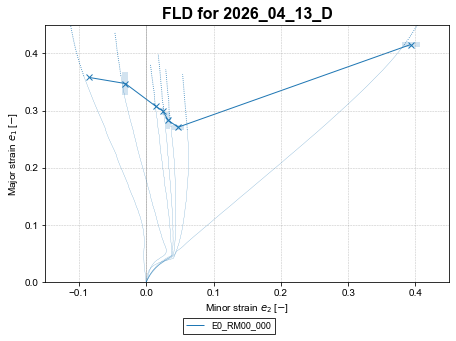
\includegraphics[width=0.75\linewidth]{report/img/FLD_example.png}
    \caption{FLC for a Serie 5 aluminum determined using the intersection line method.}
    \label{fig:FLD_example}
\end{figure}

\section{Nakazima and Marciniak Tests}
The Nakazima and Marciniak tests are the two most commonly used experimental methods for determining Forming Limit Curves (FLCs). Both tests aim to generate different strain paths by varying the specimen geometry, thereby covering the range from uniaxial tension to equi-biaxial strains required for constructing a complete Forming Limit Diagram (FLD).

In the Nakazima test, a hemispherical punch is driven into a clamped sheet specimen until localized necking or fracture occurs. Different strain paths are obtained by varying the specimen width, with narrow specimens approaching uniaxial tension and wider specimens approaching equi-biaxial stretching. Due to the direct contact between the punch and the specimen, the deformation is influenced by bending and contact pressure effects, which can lead to slightly non-linear strain paths at the specimen apex~\cite{ISO120042}.

The Marciniak test employs a flat-bottomed cylindrical punch together with a carrier blank positioned between the punch and the specimen. This arrangement prevents direct contact between the punch and the investigated sheet and promotes failure in a region of more homogeneous deformation. As a result, the Marciniak configuration generally produces more linear strain paths than the Nakazima test and is often considered more suitable for fundamental investigations of forming limits~\cite{ISO120042, Min2017}.

While ISO~12004-2 specifies a reference punch diameter of 100\,mm for both testing methods, the present work additionally investigates the influence of punch geometry by considering hemispherical punch diameters of 40\,mm, 60\,mm, 80\,mm, and 100\,mm in the Nakazima configuration. This enables a systematic assessment of the influence of punch size on the measured forming limits and contributes to the broader investigation of size effects in sheet metal forming.


\section{Punch-in-Punch Test}

The Punch-in-Punch (PiP) test is an alternative forming test designed to generate more linear strain paths than the standard Nakazima configuration, particularly in the biaxial stretching regime. It employs two coaxial punches acting sequentially on the specimen:

The process consists of two steps. In Step~1, both punches advance together, pre-forming the specimen. In Step~2, the outter punch is held fixed while the inner one advances further, deepening the dome until fracture. This two-stage loading produces a more controlled strain path.

\section{Forming Limit Identification Methods}


Determining the onset of localised necking from strain field data is non-trivial. Several criteria have been proposed in the literature, each based on different physical assumptions. .

\subsection{ISO 12004-2 Position-Dependent Method}

The standard method in ISO~12004-2~\cite{ISO120042} fits an inverse parabola to the cross-sectional strain profile perpendicular to the crack at the last frame before fracture. The FLC point is extrapolated from the fit at the section centre. The method requires spatial strain data (DIC or printed grid) and is position-dependent. For materials with unstable strain localisation or dynamic strain ageing, the selected evaluation frame and section can strongly influence the result, motivating the more robust automated criteria addressed in Task~II.

\subsection{Volk-Hora Time-Dependent Method}

Volk and Hora~\cite{VolkHora2011} proposed a fully automatic, time-dependent algorithm that identifies necking onset from the evolution of the strain distribution and its time derivatives. Necking is detected from a 2D analysis of strain localisation without relying on a single cross-section, making the method more robust and user-independent than the ISO procedure.

\subsection{Merklein Time-Dependent Method}

Merklein et al.~\cite{Merklein2010} introduced a time-dependent regression method that detects necking by fitting a polynomial to the time evolution of the major strain at the critical point. The onset is identified when the strain rate deviates significantly from the pre-necking trend, independently of the strain state.

\subsection{Pham-Sigvant Method}

Pham et al.~\cite{Pham2023} proposed a method based on the coefficient of variation of the DIC strain field over a local neighbourhood. Necking onset is defined by a threshold on this quantity. The method was validated on DP800 steel and AA6016 aluminium and yields consistently lower FLC values than ISO and time-dependent methods.

\subsection{Min-Stoughton Curvature Method}

Min et al.~\cite{Min2017} developed a curvature-based criterion that detects necking from the second derivative of the major strain in time or space. Originally designed for Marciniak tests, it was extended to Nakazima tests with corrections for the non-linear strain path effects introduced by the hemispherical punch.
